
\nobreak We've only just scratched the surface of sequences, and
already we've arrived in Chapter~\xrefn{chapter:series}.  Series will
be the main focus of our attention for the rest of the course.  If
that's the case, then why did we bother with sequences?  Because
\textbf{a series is what you get when you add up the terms of a
  sequence, \textit{in order}}.  So we needed to talk about sequences
to provide the language with which to discuss series.

Suppose $(a_n)$ is a sequence; then the associated series\sidenote{The
  $\Sigma$ symbol may look like an E, but it is the Greek letter
  \textit{sigma}, and it makes an S sound---just like the first letter
  of the word ``series.''  If you see ``GR$\Sigma\Sigma$K,'' say ``grssk.''}
$$\sum_{k=1}^\infty a_k=a_1+a_2+a_3+a_4+a_5+\cdots$$
I might be thinking that I feel just fine, but I have woken a terrible
beast!  What does that innocuous looking ``$\cdots$'' mean?  What does
it mean to add up infinitely many numbers?  It's not as if I'll ever
be done with all the adding, so how can I ever attach a ``value'' to a
series?  How can I do infinitely many things, yet live to share the
answer with you?

I can't.

But I can do a large, but finite, number of things, and then see if
I'm getting close to anything in particular.  In other words, I can
take a limit.

\section{Definition of convergence}
\label{section:series-definition}

But a limit\ldots of what?  From a sequence, we can consider the
associated series, and associated to that series is a yet another
sequence---the \defnword{sequence of partial sums}\index{sequence!of
  partial sums}\index{partial sums}.  Here's a formal definition which unwinds this tangled web.
\begin{definition}
  Suppose $(a_n)$ is a sequence with associated series
  $\ds\sum_{k=1}^\infty a_k$.  The \defnword{sequence of partial sums}
  associated to these objects is the sequence
 $$
 s_n = \sum_{k=0}^n a_k.
 $$
 \end{definition}
Working this out, we have
\begin{align*}
  s_1&=a_1, \\
  s_2&=a_1+a_2,\\ 
  s_3&=a_1+a_2+a_3, \\
  s_4&=a_1+a_2+a_3+a_4, \\
  s_5&=a_1+a_2+a_3+a_4+a_5, \mbox{ and so on.}\\
\end{align*}
Instead of adding up the infinite sequence $a_n$, which we can't do,
we will instead look at the sequence of partial sums, and ask whether
that sequence of partial sums converges.  And if it converges to $L$,
then we'll call $L$ the \defnword{value}\index{series!value of}\index{value of series} of the series.

\marginnote{This might seem overly complicated, but it solves a serious problem: we no longer are confronted with the \href{http://en.wikipedia.org/wiki/Supertask}{supertask} of adding up infintely many numbers but living to tell the tale.  To take the limit of the sequence of partial sums \textit{is} to add up lots---but not all!---of the terms in the original sequence to see if we're staying close to a particular number---the limit.  That particular limiting value is then, by definition, \textit{declared} to be the result of adding up all the terms in the original sequence \textit{in order.}}

\marginnote{That the order matters will be a major theme in Chapter~\xrefn{chapter:alternating-series}.}

\begin{definition}
Consider the series $\ds\sum_{k=1}^\infty a_k$.  This series \defnword{converges}\index{series!convergent}\index{convergent series} 
if the sequence of partial sums $s_n = \sum_{k=0}^n a_k$ converges.  More precisely, if $\ds\lim_{n \to \infty} s_n = L$, we then write
$$
\sum_{k=1}^\infty a_k = L
$$
and say, ``the series $\ds\sum_{k=1}^\infty a_k$ converges to $L$.''

If the sequence of partial sums diverges, we say that the series \defnword{diverges}\index{series!divergent}\index{divergent series}.
\end{definition}

Remember, infinity is not a number.  So if it happens that $\ds\lim_{n
  to \infty} \sum_{k=1}^n a_k = \infty$, then we might write
$\sum_{k=1}^\infty a_k = \infty$ but nevertheless we still say that
the series diverges.

\marginnote{Sometimes, to emphasize that the series involves adding up
  infinitely many terms, we will say \defnword{``infinite
    series''}\index{infinite series|see{series}} instead of just
  ``series.''}

\section{Geometric series}
\label{section:geometric-series}

Armed with the official definition of convergence in general, we focus
in on the specific example: a sequence of the form $a_n= a_0 \, r^n$
is called an \defnword{geometric progression} as we learned back in
Subsection~\xrefn{subsection:geometric-sequences}.  What happens when
we add up the terms of a geometric progression?

\marginnote{A geometric series was used by Archimedes---who lived more
  than two thousand years ago!---to compute
  \href{http://en.wikipedia.org/wiki/The_Quadrature_of_the_Parabola}{the
    area between a parabola and a straight line.}  Humans had the
  first inklings of calculus a very long time ago.}

\begin{definition}[Geometric Series]
A series of the form
$$
\ds\sum_{k=0}^\infty a_0 \, r^k
$$
is called a \defnword{geometric series}\index{geometric
  series}\index{series!geometric}.
\end{definition}

We can't simply ``add'' up the infinitely many terms in the geometric
series.  What we can do, instead, is add up the a first handful of
terms.  Pick a big value for $n$, and instead compute
$$
s_n = \ds\sum_{k=0}^n a_0\, r^k = a_0\, +a_0\, r+a_0\, r^2+a_0\, r^3+\cdots+a_0\, r^n.
$$
This is the $n^{\nth}$ partial sum.  Concretely,
\begin{align*}
s_0 &= a_0, \\
s_1 &= a_0 + a_0\, r, \\
s_2 &= a_0 + a_0\, r + a_0 \, r^2, \\
s_3 &= a_0 + a_0\, r + a_0 \, r^2 + a_0 \, r^3 \\
& \vdots \\
s_n &= a_0\, +a_0\, r+a_0\, r^2+a_0\, r^3+\cdots+a_0\, r^n.
\end{align*}
In our quest to assign a value to the infinite series
$\ds\sum_{k=0}^\infty a_0 \, r^k$, we instead\sidenote{Replacing the
  actual ``$\infty$'' by a limit (that is, a ``potential'' infinity)
  shouldn't seem all that surprising; we encountered the same trick
  in Calculus One.} consider
$$
\lim_{n \to \infty} s_n = \lim_{n \to \infty} \ds\sum_{k=0}^n a_0 \, r^k.
$$
We can perform some algebraic manipulations on the partial sum.
The manipulation begins with our multiplying $s_n$ by $(1-r)$ to cause some
convenient cancellation, specifically,
\begin{align*}
  s_n(1-r) &= a_0\, (1+r+r^2+r^3 + \cdots + r^n) \, (1-r) \\
  &=a_0\, (1+r+r^2+r^3+\cdots+r^n) \, 1 - a_0\, (1+r+r^2+r^3+\cdots+r^{n-1}+r^n)\, r \\
  &=a_0\, (1+r+r^2+r^3+\cdots+r^n) - a_0\, (r+r^2+r^3+\cdots+r^{n-1}+r^{n+1}) \\
  &=a_0 \, (1+r+r^2+r^3+\cdots+r^n-r-r^2-r^3-\cdots-r^n-r^{n+1}) \\
  &=a_0(1-r^{n+1}). \\
\end{align*}
Dividing both sides\sidenote{Here, we tacitly assume $r \neq 1$.  But can you see what happens to the geometric series when $r = 1$ without going through this argument?} by $(1-r)$ shows
$$
s_n = a_0 \cdot \frac{1 - r^{n+1}}{1-r}.
$$
Therefore,
$$
\sum_{k=0}^\infty a_0 \, r^k = \lim_{n \to \infty} s_n = \lim_{n \to \infty} \left( a_0 \cdot \frac{1 - r^{n+1}}{1-r} \right).
$$
The limit depends very much on what $r$ is.

Suppose $r \geq 1$ or $r \leq -1$.  In those cases, $\ds\lim_{n \to
  \infty} r^{n+1}$ does not exist, and likewise $\ds\lim_{n \to
  \infty} s_n$ does not exist.  So the series diverges if $r \geq 1$
or if $r \leq -1$.  One quicker way of saying this is that the series
diverges when $|r| \geq 1$.

On the other hand, suppose $|r| < 1$.  Then $\ds\lim_{n\to\infty} r^{n+1}=0$, and so
$$
  \lim_{n\to\infty}s_n=\lim_{n\to\infty}a_0{1-r^{n+1}\over 1-r}=
  \frac{a_0}{1-r}.
$$ 
Thus, when $|r|<1$ the geometric series converges to $a_0/(1-r)$.   This is important enough that we'll summarize it as a theorem.

\begin{theorem}\label{thm:geometric-series}
  Suppose $a_0 \neq 0$.  Then for a real number $r$ such that $|r| < 1$, the geometric series
  $$
  \sum_{k=0}^\infty a_0 r^k
  $$
  converges to $\ds\frac{a_0}{1-r}$.

  For a real number $r$ where $|r| \geq 1$, the aforementioned
  geometric series diverges.
\end{theorem}

\begin{example}
\label{example:sum-of-half-powers}
  When, for example, $a_0=1$ and $r=1/2$, this means
$$
\sum_{k=0}^\infty \left( \frac{1}{2} \right)^k = \frac{1}{1 - \frac{1}{2}} = 2,
$$
which makes sense.  Consider the partial sum
$$
s_n = 1 + \frac{1}{2} 
 + \frac{1}{4} 
 + \frac{1}{8} 
 + \frac{1}{16}  + \cdots + \frac{1}{2^n}.
$$
This partial sum gets as close to two as you'd like---as long as you are willing to choose $n$ large enough.  And it doesn't take long to get close to two!  For example, even just $n=6$, we get
$$
s_6 = 
1
+ \frac{1}{2} 
+ \frac{1}{4} 
+ \frac{1}{8} 
+ \frac{1}{16} 
+ \frac{1}{32} 
+ \frac{1}{64} = \frac{127}{64}
$$
which is close to two.
\end{example}

\begin{marginfigure}
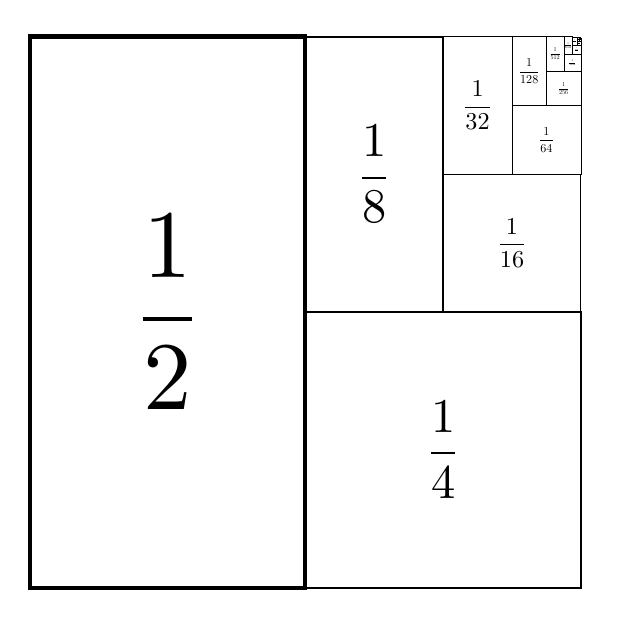
\begin{tikzpicture}[x=7cm,y=7cm]

    \draw[line width=0.75000pt] (0.50000, 0.00000) rectangle (1.0,0.50000);
  \node[anchor=center] (2) at (0.75000,0.25000) {\scalebox{1.75000}{$\displaystyle\frac{1}{4}$}};
    \draw[line width=0.37500pt] (0.75000, 0.50000) rectangle (1.0,0.75000);
  \node[anchor=center] (3) at (0.87500,0.62500) {\scalebox{0.87500}{$\displaystyle\frac{1}{16}$}};
    \draw[line width=0.18750pt] (0.87500, 0.75000) rectangle (1.0,0.87500);
  \node[anchor=center] (4) at (0.93750,0.81250) {\scalebox{0.43750}{$\displaystyle\frac{1}{64}$}};
    \draw[line width=0.09375pt] (0.93750, 0.87500) rectangle (1.0,0.93750);
  \node[anchor=center] (5) at (0.96875,0.90625) {\scalebox{0.21875}{$\displaystyle\frac{1}{256}$}};
    \draw[line width=0.04688pt] (0.96875, 0.93750) rectangle (1.0,0.96875);
  \node[anchor=center] (6) at (0.98438,0.95312) {\scalebox{0.10938}{$\displaystyle\frac{1}{1024}$}};
    \draw[line width=0.03pt] (0.98438, 0.96875) rectangle (1.0,0.98438);
  \node[anchor=center] (7) at (0.99219,0.97656) {\scalebox{0.05469}{$\displaystyle\frac{1}{4096}$}};
    \draw[line width=0.03pt] (0.99219, 0.98438) rectangle (1.0,0.99219);
  \node[anchor=center] (8) at (0.99609,0.98828) {\scalebox{0.02734}{$\displaystyle\frac{1}{16384}$}};
    \draw[line width=0.03pt] (0.99609, 0.99219) rectangle (1.0,0.99609);
  \node[anchor=center] (9) at (0.99805,0.99414) {\scalebox{0.01367}{$\displaystyle\frac{1}{65536}$}};
    \draw[line width=0.03pt] (0.99805, 0.99609) rectangle (1.0,0.99805);
  \node[anchor=center] (10) at (0.99902,0.99707) {\scalebox{0.00684}{$\displaystyle\frac{1}{262144}$}};

    \draw[line width=1.50000pt] (0.00000, 1.00000) rectangle (0.50000,0.00000);
  \node[anchor=center] (1) at (0.25000,0.50000) {\scalebox{3.50000}{$\displaystyle\frac{1}{2}$}};
    \draw[line width=0.75000pt] (0.50000, 1.00000) rectangle (0.75000,0.50000);
  \node[anchor=center] (2) at (0.62500,0.75000) {\scalebox{1.75000}{$\displaystyle\frac{1}{8}$}};
    \draw[line width=0.37500pt] (0.75000, 1.00000) rectangle (0.87500,0.75000);
  \node[anchor=center] (3) at (0.81250,0.87500) {\scalebox{0.87500}{$\displaystyle\frac{1}{32}$}};
    \draw[line width=0.18750pt] (0.87500, 1.00000) rectangle (0.93750,0.87500);
  \node[anchor=center] (4) at (0.90625,0.93750) {\scalebox{0.43750}{$\displaystyle\frac{1}{128}$}};
    \draw[line width=0.09375pt] (0.93750, 1.00000) rectangle (0.96875,0.93750);
  \node[anchor=center] (5) at (0.95312,0.96875) {\scalebox{0.21875}{$\displaystyle\frac{1}{512}$}};
    \draw[line width=0.04688pt] (0.96875, 1.00000) rectangle (0.98438,0.96875);
  \node[anchor=center] (6) at (0.97656,0.98438) {\scalebox{0.10938}{$\displaystyle\frac{1}{2048}$}};
    \draw[line width=0.03pt] (0.98438, 1.00000) rectangle (0.99219,0.98438);
  \node[anchor=center] (7) at (0.98828,0.99219) {\scalebox{0.05469}{$\displaystyle\frac{1}{8192}$}};
    \draw[line width=0.03pt] (0.99219, 1.00000) rectangle (0.99609,0.99219);
  \node[anchor=center] (8) at (0.99414,0.99609) {\scalebox{0.02734}{$\displaystyle\frac{1}{32768}$}};
    \draw[line width=0.03pt] (0.99609, 1.00000) rectangle (0.99805,0.99609);
  \node[anchor=center] (9) at (0.99707,0.99805) {\scalebox{0.01367}{$\displaystyle\frac{1}{131072}$}};
    \draw[line width=0.03pt] (0.99805, 1.00000) rectangle (0.99902,0.99805);
  \node[anchor=center] (10) at (0.99854,0.99902) {\scalebox{0.00684}{$\displaystyle\frac{1}{524288}$}};

\end{tikzpicture}
\caption{Visual evidence that $\ds\sum_{n=1}^\infty \frac{1}{2^n} =
  1$.  Begin with a $\ds \frac{1}{2} \times 1$ rectangle, and build
  each subsequent rectangle by cloning and halving the previous
  rectangle; all these rectangles fit together to fill up a unit
  square.}
\label{fig:visual-proof-geometric-series}
\end{marginfigure}

\begin{example}
Consider the series 
$$\sum_{k=1}^\infty {1\over 2^k}.$$
This does not \textit{quite} fit into the preceding framework, because
this series starts with $k = 1$ instead of $k = 0$.  

Nevertheless, we can work out what happens.  The series
$\ds\sum_{k=1}^\infty {1\over 2^k}$ is just like series
$\ds\sum_{k=0}^\infty \frac{1}{2^k}$ except the former is missing an
initial $k = 0$ term, which is $1/2^0 = 1$.  So each partial sum of
the former series is one less than the corresponding partial sum for
the latter series, so the limit is also one less than the value of the
geometric series.  In symbols,
$$
\sum_{n=1}^\infty {1\over 2^n} = \left( \sum_{n=0}^\infty {1\over 2^n} \right) - 1 = \frac{1}{1 - \frac{1}{2}} - 1 = 1.
$$
If you don't find this argument convincing, look at
Figure~\xrefn{fig:visual-proof-geometric-series}, which displays a
visual argument that the series $\ds\sum_{k=1}^\infty \frac{1}{2^k}$
converges to one.
\end{example}

\section{Properties of series}

Theorem~\xrefn{thm:properties-of-sequences} presented many properties
of sequences.  Since the value of a series is the limit of the
sequence of partial sums, properties of limits can be reformulated
into properties of series.

\subsection{Constant multiple}

\begin{theorem} \relax\label{thm:series-are-linear}
Suppose $\sum_{k=0}^\infty a_k$ is a convergent series, and $c$ is a constant. Then $\ds\sum_{k=0}^\infty c\,a_k$ converges, and
$$\ds\sum_{k=0}^\infty c\,a_k=c\sum_{k=0}^\infty a_k.$$
\end{theorem}

\begin{proof}
  If you know just enough algebra to be dangerous, you may remember
  that for any real numbers $a$, $b$, and $c$,
  $$
  c(a+b) = c \, a + c \, b.
  $$
  This is the \defnword{distributive law}\index{distributive law} for
  real numbers.  By using the distributive law more than once, 
  $$
  c(a_0+a_1+a_2) = c \, a_0  + c \, a_1 + c \, a_2,
  $$
  or more generally, for some finite $n$,
  $$
  c(a_0+a_1+a_2 + \cdots + a_n) = c \, a_0  + c \, a_1 + c \, a_2 + \cdots + c \, a_n.
  $$
  So what's the big deal with proving
  Theorem~\label{thm:distributive-over-series}?  Can't we just scream
  ``distributive law!'' and be done with it?  After all,
  Theorem~\label{thm:distributive-over-series} amounts to 
  $$
  c \, a_0  + c \, a_1 + c \, a_2 + \cdots + c \, a_n + \cdots = c(a_0+a_1+a_2 + \cdots + a_n + \cdots ).
  $$
  But hold your horses: you can only apply the distributive law
  \textit{finitely} many times!  The distributive law, without some
  input from calculus, will not succeed in justifying
  Theorem~\label{thm:distributive-over-series}.

  Let's see how to handle this formally.  By hypothesis,
  $\sum_{k=0}^\infty a_k$ is a convergent series, meaning its associated sequence of partial sums,
  $$
  s_n = \sum_{k=0}^n a_k,
  $$
  converges.  In other words, $\ds\lim_{n \to \infty} s_n$ exists.  Then, by Theorem~\label{thm:distributive-over-series},
  $$
  \lim_{n \to \infty} (c\, s_n) = c \, \lim_{n \to \infty} s_n.
  $$
  But $c \, s_n$ is the sequence of partial sums for the series $\ds\sum_{k=0}^\infty c \, a_k$, because
  $$
  c \, s_n = c\, a_0 + c\, a_1 + c \, a_2 + \cdots + c \, a_n.
  $$
  Consequently,
  $$ 
  \ds\sum_{k=0}^\infty c \, a_k = \lim_{n \to \infty} (c \, s_n) = c \, \lim_{n \to \infty} s_n,
  $$
  which is what we wanted to prove.
\end{proof}

That theorem addresses the case of multiplying a convergent series by
a constant $c$; what about divergence?

\begin{example}
Suppose that $\ds\sum_{k=0}^\infty a_k$ diverges; does $\ds\sum_{k=0}^\infty c\,a_k$ also diverge?
\end{example}

\begin{solution}
  If $c = 0$, then $\ds\sum_{k=0}^\infty c\,a_k = \ds\sum_{k=0}^\infty
  0$ which does converge, to zero.

  On the other hand, provided $c \neq 0$, then, yes,
  $\ds\sum_{k=0}^\infty c\,a_k$ also diverges.  How do we know?
  
  We are working under the hypothesis that $\ds\sum_{k=0}^\infty a_k$
  diverges.  Suppose now, to the contrary, that $\sum_{k=0}^\infty
  c\,a_k$ did converge; applying Theorem~\xrefn{thm:series-are-linear}
  (albeit with $a_k$ replaced by $c\,a_k$ and $c$ replaced by
  $(1/c)$), the series
  $$\sum_{k=0}^\infty \left(\frac{1}{c} \right) \,c \, a_k $$ converges, but
  that is ridiculous, since 
  $$\sum_{k=0}^\infty \left(\frac{1}{c} \right) \,c \, a_k = \sum_{k=0}^\infty a_k$$
  and the latter, under our hypothesis, diverged.  A series cannot
  both converge and diverge, so our assumption (that
  $\sum_{k=0}^\infty c\,a_k$ did converge) must have been
  mistaken---it must be that $\sum_{k=0}^\infty c\,a_k$ diverges.
\end{solution}

But what about the case where $c = 0$?  In that case, the series
converged!  Did we make a mistake?  In the argument for divergence, we
multiplied by $1/c$, which is something we are not permitted to do
when $c = 0$.

\marginnote{We can connect this discussion back to the discussion of
  geometric series in Section~\xrefn{section:geometric-series}.  If
  you believe that $\ds\sum_{k=0}^\infty r^k = \ds\frac{1}{1-r}$, then
  by Theorem~\xrefn{thm:distributive-over-series}, you believe
  $\ds\sum_{k=0}^\infty c \, r^k = \ds\frac{c}{1-r}$, which is part of
  Theorem~\xrefn{thm:geometric-series}.}

In light of this example, we have actually proved something stronger.
\begin{theorem}\label{thm:distributive-over-series}
  Consider the series $\sum_{k=0}^\infty a_k$, and suppose $c$ is a
  nonzero constant.  Then $\sum_{k=0}^\infty a_k$ and
  $\sum_{k=0}^\infty c\,a_k$ share a common fate: either both series
  converge, or both series diverge.

  Moreover, when $\ds\sum_{k=0}^\infty a_k$ converges,
  $$
  \sum_{k=0}^\infty c \, a_k = c \cdot \sum_{k=0}^\infty a_k.
  $$
\end{theorem}

\subsection{Sum of series}

Suppose $\sum_{k=0}^\infty a_k$ and $\sum_{k=0}^\infty b_k$ are
convergent series. What can be said of $\ds\sum_{k=0}^\infty
(a_k+b_k)$?

Addition is \defnword{associative}\sidenote{To say that addition is
  ``associative'' is, intuitively, to say that how the expression is
  parenthesized doesn't matter; formally, ``associativity'' means
  that for any $a$, $b$, and $c$, we have $a + (b+c) = (a+b) +
  c$.}\index{associativity} and \defnword{commutative}\sidenote{To
  say that addition is ``commutative'' is, intuitively, to say that
  the order in which the adding is done doesn't matter; formally,
  ``commutativity'' means that for $a$ and $b$, we have $a + b =
  b+a$.}\index{commutativity}, so for any real numbers $a$, $b$,
$c$, and $d$,
$$
(a+b)+(c+d) = (a+c) + (b+d).
$$
More generally, for real numbers $a_0$, $a_1$, $a_2$, \ldots, $a_n$ and real numbers
$b_0$, $b_1$, $b_2$, \ldots, $b_n$,
$$
(a_0 + a_1 + a_2 + \cdots + a_n)+(b_0 + b_1 + b_2 + \cdots + b_n) = (a_0 + b_0) + (a_1 + b_1) + (a_2 + b_2) + \cdots + (a_n + b_n).
$$
But this finite statement can be beefed up into a statement about series.  What we want to prove is
$$
\sum_{k=0}^\infty a_k + \sum_{k=0}^\infty b_k = \sum_{k=0}^\infty \left( a_k + b_k \right).
$$
From above, we already know
$$
\sum_{k=0}^n a_k + \sum_{k=0}^n b_k = \sum_{k=0}^n \left( a_k + b_k \right).
$$
Take the limit of both sides.
$$
\lim_{n \to \infty} \left( \sum_{k=0}^n a_k + \sum_{k=0}^n b_k \right) = \lim_{n \to \infty} \sum_{k=0}^n \left( a_k + b_k \right).
$$
But the limit of a sum is the sum of the limits\sidenote{I like to call this a \defnword{chiastic rule}\index{chiastic rule}, since it has the rhetorical pattern of a \href{http://en.wikipedia.org/wiki/Chiasmus}{chiasmus}.}, so
$$
\left( \lim_{n \to \infty} \sum_{k=0}^n a_k \right) + \left( \lim_{n \to \infty} \sum_{k=0}^n b_k \right) = \lim_{n \to \infty} \sum_{k=0}^n \left( a_k + b_k \right).
$$
Those three limits of partial sums can each be replaced by the series, which shows
$$
\sum_{k=0}^\infty a_k + \sum_{k=0}^\infty b_k = \sum_{k=0}^\infty \left( a_k + b_k \right).
$$
This can be summarized in a theorem.
\begin{theorem} \relax\label{thm:series-are-linear}
  Suppose $\sum_{k=0}^\infty a_k$ and $\sum_{k=0}^\infty b_k$ are
  convergent series. Then $\ds\sum_{k=0}^\infty (a_k+b_k)$ is
  convergent, and
$$\ds\sum_{k=0}^\infty (a_k+b_k)=\left( \sum_{k=0}^\infty a_k \right)+\left(\sum_{k=0}^\infty b_k\right).$$
\end{theorem}
That covers sums of convergent series.

\begin{example}
Now suppose that $\sum_{k=0}^\infty a_k$ and $\sum_{k=0}^\infty b_k$ diverge; does
$\sum_{k=0}^\infty (a_k+b_k)$ diverge?
\end{example}

\begin{solution}
  Not necessarily.  Let $a_k=1$ and $b_k=-1$, so $\sum_{k=0}^\infty
  a_k$ and $\sum_{k=0}^\infty b_k$ diverge. But
$$\sum_{k=0}^\infty (a_k+b_k)=\sum_{k=0}^\infty \left( \left( 1 \right) + \left( -1 \right) \right)=\sum_{k=0}^\infty 0 = 0.
$$
This is \textit{not} to say that the term-by-term sum of divergent
series \textit{necessarily} converges, either.  It is entirely
possible that $\sum_{k=0}^\infty (a_k+b_k)$ will also diverge.  For
istance, if $a_k=b_k=1$, then 
$$\sum_{k=0}^\infty (a_k+b_k)=\sum_{k=0}^\infty(1+1)=\sum_{k=0}^\infty 2
$$
also diverges.  So the term-by-term sum of divergent series might
converge or might diverge, depending on the situation.
\end{solution}

%%%%%%%%%%%%%%%%%%%%%%%%%%%%%%%%%%%%%%%%%%%%%%%%%%%%%%%%%%%%%%%%
\section{Telescoping series}
\label{section:telescoping-series}

For most of this course, we will be happy if we can show that a series
converges or that a series diverges; we will not, usually, be too
concerned with finding the value of a series.  Why not?  Usually it is
just too hard to determine the value; we would if we could, but since
it is often too hard, we don't bother.

Nevertheless, there is one family of series for which we can calculate
the value with relative ease: the \defnword{telescoping series.}  Here
is a first example which suggests what we mean by ``telescoping.''

\begin{example}
Compute $\sum_{k=1}^n \frac{1}{k \cdot (k+1)}$.
\end{example}

\begin{solution}
  Doing some algebra verifies that
  $$
  \frac{1}{k \cdot (k+1)} = \frac{1}{k} - \frac{1}{k+1}
  $$
  Consequently,
\begin{align*}
\sum_{k=1}^n \frac{1}{k \cdot (k+1)} &=
\left( \frac{1}{1} - \frac{1}{1+1} \right) + 
\left( \frac{1}{2} - \frac{1}{2+1} \right) + 
\left( \frac{1}{3} - \frac{1}{3+1} \right) + \cdots + 
\left( \frac{1}{n} - \frac{1}{n+1} \right) \\
&=
\frac{1}{1} +
\left( - \frac{1}{1+1} \frac{1}{2} \right) + 
\left(- \frac{1}{2+1} + \frac{1}{3} \right) + \cdots + 
\left( - \frac{1}{(n-1)+1} + \frac{1}{n} \right) 
- \frac{1}{n+1} \\
&= \frac{1}{1} - \frac{1}{n+1}
\end{align*}
since most of these terms end up canceling.
\end{solution}

In general, we say that a series
\defnword{telescopes}\index{series!telescoping}\index{telescoping
  series} if, after some simplification, there is a formula for
the sequence of partial sums with a fixed number of terms.  The name
suggests the way the cancellation happens: just as the nesting rings
in an expandable spyglass fit together, so too do the neighboring
terms in a telescoping series fit together and collapse.

Armed with a formula for the sequence of partial sums, we can attack the corresponding infinite series.

\begin{example}
Compute $\sum_{k=1}^\infty \frac{1}{k \cdot (k+1)}$.
\end{example}
\begin{solution}
We just computed that
$$
\sum_{k=1}^n \frac{1}{k \cdot (k+1)} = 1 - \frac{1}{n+1}.
$$
Rewriting the infinite series as the limit of the sequence of partial sums yields
\begin{align*}
\sum_{k=1}^\infty \frac{1}{k \cdot (k+1)} &= \lim_{n \to \infty} \sum_{k=1}^n \frac{1}{k \cdot (k+1)} \\
&= \lim_{n \to \infty} \left( 1 - \frac{1}{n+1} \right) \\
&= \lim_{n \to \infty} 1 - \lim_{n \to \infty} \frac{1}{n+1} \\
&= 1 - 0 = 1.\\
\end{align*}
So the value of this series is 1.
\end{solution}

%%%%%%%%%%%%%%%%%%%%%%%%%%%%%%%%%%%%%%%%%%%%%%%%%%%%%%%%%%%%%%%%
\section{A test for divergence}
\label{section:nth-term-test}

Usually, the sequence of partial sums $\ds s_n = a_0 + a_1 + \cdots +
a_n$ is harder to understand and analyze than the sequence of terms
$\ds a_k$.  It would be helpful if we could say something about the
complicated sequence $s_n$ by studying the easier-to-understand
sequence $a_k$.

Specifically, if the sequence $s_n$ converges, what can be said about
the sequence $a_k$?  If adding up more and more terms from the
sequence $a_k$ gets closer and closer to some number, then the size of
the terms of $a_k$ had better be getting very smaller.  Let's make
this precise.

\begin{theorem}\label{thm:divergence-test} If $\sum_{k=0}^\infty a_k$
  converges then $\ds\lim_{n\to\infty}a_n=0$.
\end{theorem}
\begin{proof} Intuitively, this should seem reasonable: after all, if
  the terms in the sequence $a_n$ were getting very large (that is,
  not converging to zero), then adding up those very large numbers
  would prevent the series $\sum_{k=0}^\infty a_k$ from converging.

  We can put this intuitive thinking on a firm foundation.  Say
  $\sum_{k=0}^\infty a_k$ converges to $L$, meaning
  $\ds\lim_{n\to\infty}s_n=L$.  But then also
  $\ds\lim_{n\to\infty}s_{n-1}=L$, because that sequence amounts to
  saying the same thing, but with the terms renumbered.  By
  Theorem~\xrefn{thm:properties of sequences},
$$
  \lim_{n\to\infty} (s_{n}-s_{n-1})=
  \lim_{n\to\infty} s_{n}-\lim_{n\to\infty}s_{n-1}=L-L=0.
$$
Replacing $s_n$ with $a_0+\cdots+a_n$, we get
$$
  s_{n}-s_{n-1}=(a_0+a_1+a_2+\cdots+a_n)-(a_0+a_1+a_2+\cdots+a_{n-1})
  =a_n,
$$
and therefore, $\ds\lim_{n\to\infty}a_n=0$.
\end{proof}

The contrapositive of Theorem~\xrefn{thm:divergence-test} can be used
as a divergence test\index{divergence test}.
\begin{theorem}\label{thm:nth-term-test}
Consider the series $\sum_{k=0}^\infty
a_k$. If the limit $\ds\lim_{n\to\infty}a_n$ does not exist or has a value
other than zero, then the series diverges.
\end{theorem}
We'll usually call this theorem the ``$n^{\nth}$ term test.''

\begin{warning}
  The converse of Theorem~\xrefn{thm:divergence-test} is {\em not\/}
  true: even if $\ds\lim_{n\to\infty}a_n=0$, the series could diverge.
  For an example, see Section~\xrefn{section:harmonic-series}.
\end{warning}
\sidenote{This is a \textit{very} common mistake: you might be tempted
  to show that a series converges by showing
  $\ds\lim_{n\to\infty}a_n=0$, but that doesn't work.  The $n^{\nth}$
  term test \textbf{either says ``diverges!'' or says nothing at all.}
  It is not possible to show that anything converges by using the
  $n^{\nth}$ term test.}  One analogy that can be helpful is think
about weather: whenever it is raining, it is cloudy.  Yet it is
possible for there to be clouds, even on a rainless day.  \sidenote{We
  first introduced this idea on
  Page~\pageref{sidenote:raining-converse}.}

Likewise, whenever the series $\ds\sum_{k=0}^\infty a_k$ converges
(``it is raining''), the sequence $a_k$ converges to zero (``it is
cloudy'').  If it isn't cloudy, then we can be sure it isn't
raining---and this is the statement of
Theorem~\xrefn{thm:nth-term-test}.  Let's use this ``divergence test''
to show that a particular series diverges.
\begin{example}
Show that $\ds\sum_{n=1}^\infty \frac{n}{n+1}$ diverges.
\end{example}

\begin{solution}
We apply the $n^{\nth}$ term test: all we need to do is to compute the limit
$$\lim _{n\to\infty}{n\over n+1}=1\not=0.$$
Since the limit exists but is not zero (i.e., ``it is not cloudy''),
the series must diverge (``it can't be raining.'').

Looking at the first few terms perhaps makes it clear that the series
has no chance of converging:
$${1\over2}+{2\over3}+{3\over4}+{4\over5}+\cdots$$
will just get larger and larger; indeed, after a bit longer the series
starts to look very much like $\cdots+1+1+1+1+\cdots$, and if we add
up many numbers which are very close to one, then we can make the sum
as large as we desire.
\end{solution}

%%%%%%%%%%%%%%%%%%%%%%%%%%%%%%%%%%%%%%%%%%%%%%%%%%%%%%%%%%%%%%%%
\section{Harmonic series}
\label{section:harmonic-series}

The series $\ds\sum_{n=1}^\infty {1\over n}$ has a special name.
\begin{definition}
  The series $$\ds\sum_{n=1}^\infty {1\over n} = \frac{1}{1} +
  \frac{1}{2} + \frac{1}{3} + \frac{1}{4} + \cdots$$ is called the
  \defnword{harmonic series}\index{series!harmonic}\index{harmonic series}.
\end{definition}
The main question for this section---indeed, the question which should
always be our first question anytime we see an unknown series---is the
following question:
\begin{quote}
  Does the harmonic series converge\ldots or diverge?
\end{quote}
How can we begin to explore this question?

\subsection{The limit of the terms}

\marginnote{When confronted with the question of whether a series
  diverges or converges, the first thing to check is the limit of the
  terms---if that limit doesn't exist, or does exist but equals a
  number other than zero, then the series diverges.}

In general, the easiest way to prove that a series diverges is to
apply the $n^{\nth}$ term test from Theorem~\xrefn{thm:nth-term-test}.
What does the $n^{\nth}$ term test tell us for the harmonic series?
We calculate
$$
\lim_{n \to \infty} \frac{1}{n} = 0,
$$
so the $n^{\nth}$ term test is \textit{silent}; since the limit of the
terms of the series exists and is equal to zero, the $n^{\nth}$ term
test does not tell us any information.

The harmonic series passed the first gauntlet---but that does not mean
the harmonic series will survive the whole game.  All we know is that
the harmonic does doesn't diverge for the most obvious reason, but
whether it diverges or converges is yet to be determined.

\subsection{Numerical evidence}

If you have the fortitude\sidenote{lacking fortitude, software will
  suffice} to add up the first hundred terms, you will find that
\begin{align*}
\sum_{n=1}^{100} {1\over n} &= \frac{1}{1} + \frac{1}{2} + \cdots + \frac{1}{100} \\
&= \frac{14466636279520351160221518043104131447711}{2788815009188499086581352357412492142272} \approx 5.19.
\end{align*}
If we add up the first thousand terms, we will find that
\begin{align*}
\sum_{n=1}^{1000} {1\over n} &= \frac{1}{1} + \frac{1}{2} + \cdots + \frac{1}{1000} \approx 7.49. \\
\end{align*}
If we add up the first ten thousand terms, we will find that
\begin{align*}
\sum_{n=1}^{10000} {1\over n} &= \frac{1}{1} + \frac{1}{2} + \cdots + \frac{1}{10000} \approx 9.79 \\
\end{align*}
The partial sums are getting bigger, but not very quickly.  Maybe the
series converges.  Maybe it converges to\ldots about ten?

\subsection{An analytic argument}

That numeric evidence might have made us think otherwise, but
\textbf{the harmonic series diverges.}

But in fact the partial sums do get arbitrarily large; they just get
big very, very slowly. Consider the following:
\begin{align*}
\ds 1+{1\over 2}+{1\over 3}+{1\over 4} &> 
1+{1\over 2}+{1\over 4}+{1\over
  4} = 1+{1\over 2}+{1\over 2} \\
\ds 1+{1\over 2}+{1\over 3}+{1\over 4}+
{1\over 5}+{1\over 6}+{1\over
    7}+{1\over 8} &> 
1+{1\over 2}+{1\over 4}+{1\over 4}+{1\over 8}+{1\over 8}+{1\over
    8}+{1\over 8} = 1+{1\over 2}+{1\over 2}+{1\over 2} \\
\ds 1+{1\over 2}+{1\over 3}+\cdots+{1\over16} &> 
1+{1\over 2}+{1\over 4}+{1\over 4}+{1\over 8}+\cdots+{1\over
  8}+{1\over16}+\cdots +{1\over16} =1+{1\over 2}+{1\over 2}+{1\over
  2}+{1\over 2} 
\end{align*}
\noindent
and so on. By swallowing up more and more terms we can always manage
to add at least another $1/2$ to the sum, and by adding enough of
these we can make the partial sums as big as we like. In fact, it's
not hard to see from this pattern that
$$1+{1\over 2}+{1\over 3}+\cdots+{1\over 2^n} > 1+{n\over 2},$$
so to make sure the sum is over 100, for example, we'd add
up terms until we get to around $\ds 1/2^{198}$, that is,
about $\ds 4\cdot 10^{59}$ terms.


%\subsection{Building a ``harmonic'' tower}
%BADBAD

%%%%%%%%%%%%%%%%%%%%%%%%%%%%%%%%%%%%%%%%%%%%%%%%%%%%%%%%%%%%%%%%
\section{Comparison test}
\label{section:comparison-test}

\input comparison-test

%%%%%%%%%%%%%%%%%%%%%%%%%%%%%%%%%%%%%%%%%%%%%%%%%%%%%%%%%%%%%%%%
\begin{exercises}

\begin{exercise} Explain why $\ds\sum_{n=1}^\infty {n^2\over 2n^2+1}$
diverges.
\begin{answer} $\ds\lim_{n\to\infty} n^2/(2n^2+1)=1/2$
\end{answer}\end{exercise}

\begin{exercise} Explain why $\ds\sum_{n=1}^\infty {5\over 2^{1/n}+14}$
diverges.
\begin{answer} $\ds\lim_{n\to\infty} 5/(2^{1/n}+14)=1/3$
\end{answer}\end{exercise}

\begin{exercise} Explain why $\ds\sum_{n=1}^\infty {3\over n}$
diverges.
\begin{answer} $\sum_{n=1}^\infty {1\over n}$ diverges, so $\ds\sum_{n=1}^\infty 3{1\over n}$ diverges
\end{answer}\end{exercise}

\twocol

\begin{exercise} Compute $\ds\sum_{n=0}^\infty {4\over (-3)^n}- {3\over 3^n}$. 
\begin{answer} $-3/2$
\end{answer}\end{exercise}

\begin{exercise} Compute $\ds\sum_{n=0}^\infty {3\over 2^n}+ {4\over 5^n}$. 
\begin{answer} $11$
\end{answer}\end{exercise}

\begin{exercise} Compute $\ds\sum_{n=0}^\infty {4^{n+1}\over 5^n}$.
\begin{answer} $20$
\end{answer}\end{exercise}

\begin{exercise} Compute $\ds\sum_{n=0}^\infty {3^{n+1}\over 7^{n+1}}$.
\begin{answer} $3/4$
\end{answer}\end{exercise}

\begin{exercise} Compute $\ds\sum_{n=1}^\infty \left({3\over 5}\right)^n$.
\begin{answer} $3/2$
\end{answer}\end{exercise}

\begin{exercise} Compute $\ds\sum_{n=1}^\infty {3^n\over 5^{n+1}}$.
\begin{answer} $3/10$
\end{answer}\end{exercise}

\endtwocol

\end{exercises}
